\ifx\wholebook\relax \else

\documentclass[b5paper]{ctexart}
\usepackage[nomarginpar
  %, margin=.5in
]{geometry}

\addtolength{\oddsidemargin}{-0.05in}
\addtolength{\evensidemargin}{-0.05in}
\addtolength{\textwidth}{0.1in}

\usepackage[cn]{../prelude}

\setcounter{page}{1}

\begin{document}

\title{零}

\author{刘新宇
\thanks{{\bfseries 刘新宇} \newline
  Email: liuxinyu99@hotmail.com \newline}
  }

\maketitle
\fi

\markboth{零}{数的旅程}

\ifx\wholebook\relax
\chapter{零}
\fi

\epigraph{因此“有”与“无”的真理,就是两者的统一。}{黑格尔《小逻辑》}

尽管数有超过5000年的历史,零却只有1200年的历史,是个“新生事物”。零诞生于印度,经由阿拉伯人引入欧洲。但它仅仅具有“占位符”的特殊身份,和1、2、3……其它数比起来是个“二等公民”,甚至面临被“开除数籍”的风险。

\section{质疑与否定}
零一出生就代表“无”、“没有”。印度人给它起名叫sunya,意为“空位”。所以2025中的0表示\underdot{没有}百。在西方,“无\footnote{对应的英文是void,表示虚空。}”在文化传统、宗教哲学上是负面否定的。它往往和黑暗、虚空、死亡等意象关联。而1代表\underdot{有}一个,2代表\underdot{有}两个……人们不说0,而说\underdot{没有},表示对\underdot{有}、\underdot{生存}、\underdot{实在}的否定。莎士比亚《王子复仇记》中的名句“To be or not to be, that is the question.”中译为“生存还是死亡?”人们说3只羊跑了1只羊,还有两只羊;如果再跑了两只羊,人们说没有羊,而不说有0只羊。

\begin{figure}[htbp]
 \centering
 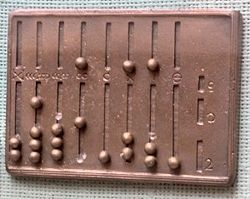
\includegraphics[scale=0.5]{img/Roman-abacus}
 \caption{现代复原的罗马算盘,在盘上开槽,槽中摆放石子,槽上标有罗马数字单位I, V, X, C, M。}
 \label{fig:roman-abacus}
 %https://www.newworldencyclopedia.org/entry/Abacus
\end{figure}

印度-阿拉伯计数系统传入欧洲后,尽管计算方便,人们还是把计算结果转换成罗马数字,而避免使用零\footnote{古代中国在进行算筹计算时(见第\ref{counting-rods}节)用空位代表0。但计算完成后就把结果用乘法分组系统表示出来,如一百、两千一十五、一百有二。汉字“零”直到宋、元后才出现。}。教会宣布0是邪恶的符号,禁止在公开场合使用。僧侣学者们用算盘(如\cref{fig:roman-abacus},不是中国明代发明的珠算)计算。欧洲的算盘源自古巴比伦的泥板。就是在一块板上用小石子按照罗马数字演算,算好后抄下结果。但商人们、银行家们看到了印度-阿拉伯数字的巨大好处,于是产生了十六世纪的“人机大战”,如\cref{fig:hindu-arabic-vs-abacus}。结果可想而知。自然是代表印度——阿拉伯计数的“机”胜了。这种“人机大战”在历史上一再上演:斯蒂芬森的火箭号列车\footnote{英国工程师乔治·斯提芬森和其子罗伯特·斯蒂芬森于1830年设计制造的蒸汽机车。}和马赛跑;深蓝挑战国际象棋大师卡斯帕罗夫;Alpha-Go挑战九段棋手李世石、柯洁;ChatGPT挑战大学生入学考试……每当有新事物出现,就有精彩的人机大战。

\begin{figure}[htbp]
 \centering
 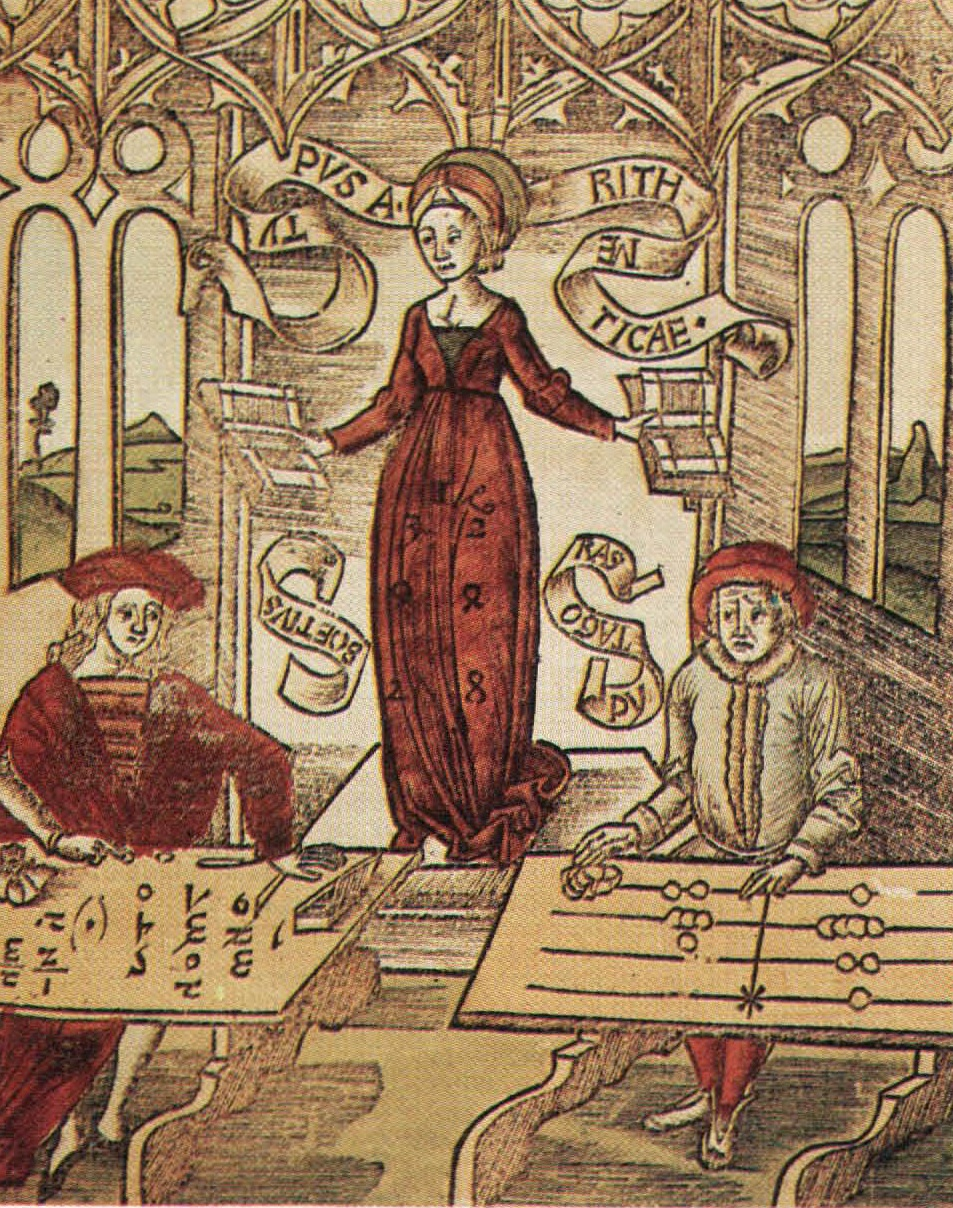
\includegraphics[scale=0.8]{img/Hindu-arabic-vs-abacus}
 \caption{1503年的版画。描绘了一个人用印度——阿拉伯数字计算,另一个人用罗马算盘计算的比赛。}
 \label{fig:hindu-arabic-vs-abacus}
 %https://www.newworldencyclopedia.org/entry/Abacus
\end{figure}

“机”的胜利让0具有了“二等公民”的身份——可以被使用了。可是为何0不能像1、2、3……那样成为“一等公民”呢?

\section{真正的数}

要想成为一等公民,0和1、2、3……比差了什么呢?是值,或者说大小。1这个符号代表的大小是1,比如1厘米的长度、1克的质量、1只羊……同样,2的值可以代表2厘米的长度、2克质量、2只羊……可是0呢?它没有值。“0是个占位符,不是一个数,因为它没有值\cite{Seife-2000}。”0极特殊,它表现得像一个破坏者,而非1、2、3……那样的“良民”。我们看看0是如何“破坏规矩”的:

\begin{enumerate}[(1)]
\item 阿基米德公理
\begin{align*}
1 + 1 &= 2   & 1 + 1 + 1 &= 3 & \dots \\
1 + 1 &= 2   & 1 + 1 + 1 &= 3 & \dots \\
1 + 1 &= 2   & 1 + 1 + 1 &= 3 & \dots \\
\dots &      & \dots     &    &
\end{align*}
一个数\footnote{本节的数都是自然数。}加上自己越来越大。阿基米德甚至指出这个规律是一个公理,今天叫做阿基米德公理:任意非零的$m < n$,则反复$m + m + \cdots$将会超过$n$。但 0 + 0 = 0没有变大,$0 + 0 + 0 + \cdots$不会超过任何数,包括1。

\item 积与面积
各个文明在丈量土地时都独立发展出了面积的概念,并将面积和乘法联系了起来。一块长方形的土地面积就是长与宽的积。长5宽1的

\begin{figure}[htbp]
 \centering
 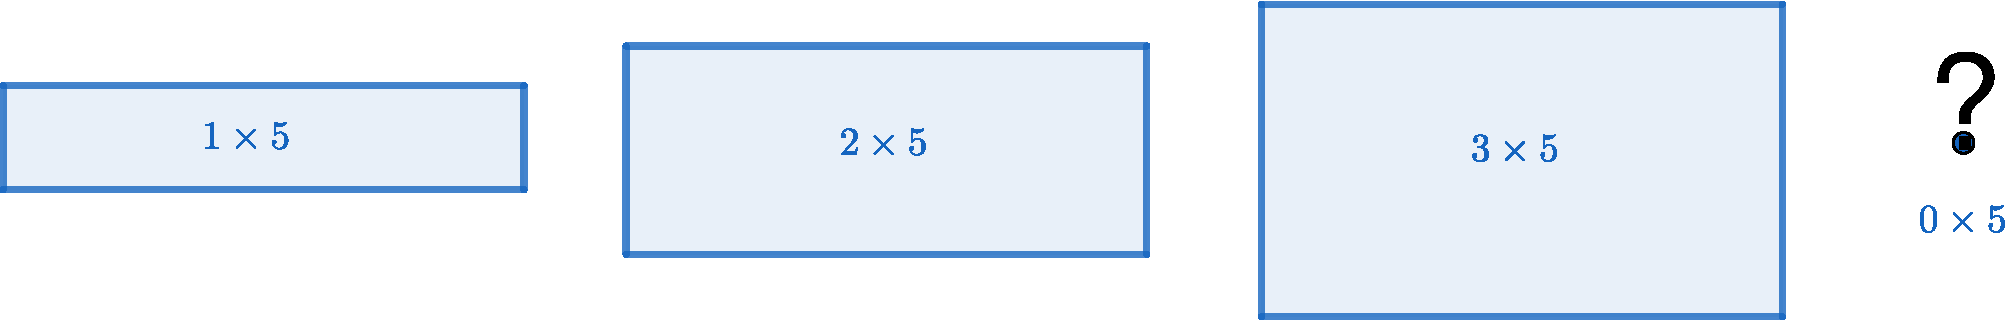
\includegraphics[scale=0.5]{img/rectangles}
 \caption{$0 \times 5$把矩形“压缩”成了一个没有大小的点。}
 \label{fig:rectangle-vanish}
\end{figure}

\end{enumerate}

\ifx\wholebook\relax \else
\section{参考答案}
\shipoutAnswer


\begin{thebibliography}{99}

\bibitem{Seife-2000}
Charles Seife. ``Zero: the biography of a number'' Penguin Books, 2000. ISBN: 9-781-1011-9960-2

\end{thebibliography}

\expandafter\enddocument
\fi
